  Logo abaixo são apresentados os resultados da segunda iteração de avaliação do protótipo de alta fidelidade,
  seguindo o planejamento realizado.
  
  \begin{itemize}
    \item \textbf{Descrição e metodologia do roteiro da avaliação}
    
    \subitem O objetivo da avaliação era analisar qual a satisfação obtida pelo usuário ao utilizar o protótipo, 
    considerando as seguintes metas:
    
    \begin{itemize}
      \item Utilidade;
	\subitem Avaliada pela dimensão \textit{SysUse} do questionário PSSUQ.
	
      \item Eficácia e eficiência;
	\subitem Avaliada pelas dimensões \textit{SysUse} e \textit{InfoQual} do questionário PSSUQ.
	
      \item Interface esteticamente agradável.
	\subitem Avaliada pela dimensão \textit{InterQual} do questionário PSSUQ.
    \end{itemize}
    
    \item \textbf{Comportamento dos usuários}
    
    \subitem Nesta iteração os usuários  agora estavam conseguindo apertar nos botões, pois eles foram aumentados. O que ocorreu é 
    que a funcionalidade de adicionar um tema ainda não estava intuitiva. O botão "+" estava passando despercebido pelos 
    usuários, mesmo este estando maior. Isso fazia com que os usuários não conseguissem prosseguir com a realização da
    funcionalidade de maneira rápida.
    
    
    \item \textbf{Resumo das entrevistas}
    
      \subitem As entrevistas foram realizadas na própria universidade. Estas foram gravadas e cada uma durou em 
	  média 10 minutos contando com o tempo que o usuário teve pra responder os questionários de avaliação.
	  
	  Os usuários deram \textit{feedback} positivo nas entrevistas com as sugestões 
	    
    \item \textbf{Problemas de usabilidade identificados}
    
      \subitem ícone de adicionar o tema da notificação não estava tão intuitivo para o usuário.
          
    \item \textbf{Paradas críticas}
    
      \subitem Não houveram paradas críticas nas avaliações realizadas.
    
    \item \textbf{Plano de correção}
    
      \subitem Para a terceira versão do protótipo, ao invés de apenas um botão de adicionar o tema da notificação, 
      agora cada tema terá em sua frente um ícone. Desta maneira, a equipe de avaliadores acredita que os usuários 
      conseguirão entender de maneira mais rápida como que se adiciona um tema.
    
  \end{itemize}
  
  Na figura \ref{asqalta_2} se encontram as respostas ao questionário ASQ pelos cinco usuários avaliados.
  
  Na figura \ref{pssuqalta_2} se encontram as respostas ao questionário PSSUQ pelos cinco usuários avaliados.
  
  \begin{figure}[!htb]
  \centering
  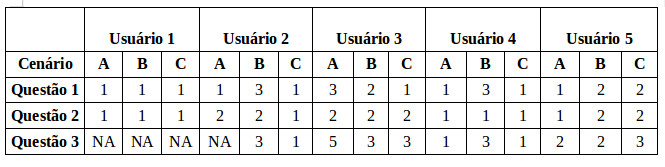
\includegraphics[scale=0.6]{figuras/asqalta_2.jpg}
  \caption{Resposta dos usuários ao questionário ASQ na segunda avaliação do protótipo de alta fidelidade}
  \label{asqalta_2}
  \end{figure}
   
  
  \begin{figure}[!htb]
  \centering
  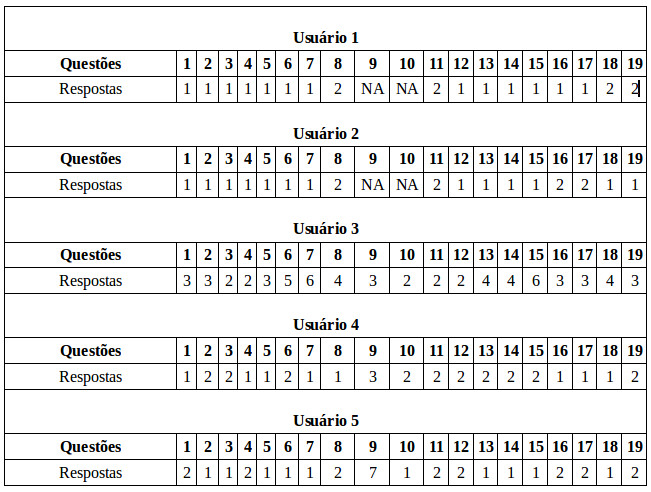
\includegraphics[scale=0.6]{figuras/pssuqalta_2.jpg}
  \caption{Resposta dos usuários ao questionário PSSUQ na segunda avaliação do protótipo de alta fidelidade}
  \label{pssuqalta_2}
  \end{figure}  